%!TEX root = ../thesis.tex
% ******************************* Thesis Appendix A ****************************
\chapter{Additional Machine Learning SVM Plots} 

\begin{figure}[!h]
\centering
\begin{minipage}{.45\textwidth}
  \centering
  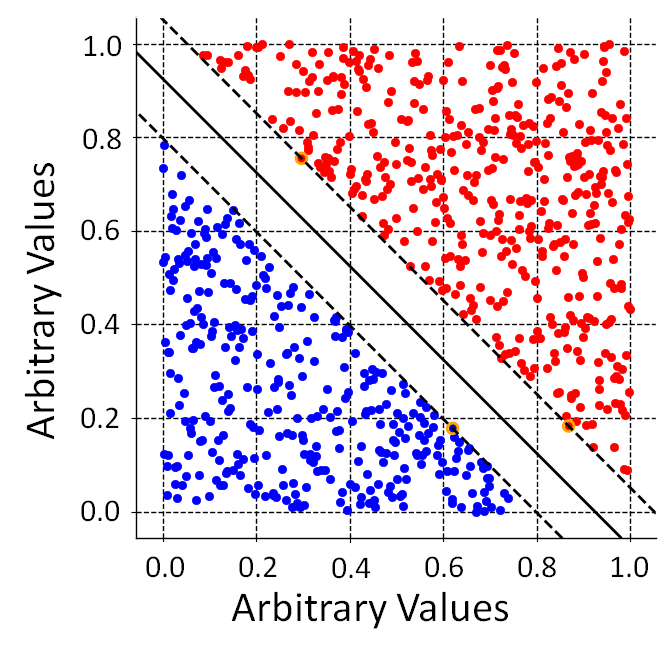
\includegraphics[width=\linewidth]{Chapter4/Figs/adjustedSvmPlots/adjusted_LinSepExample.png}
  \captionof{figure}[LIBSVM linear separation example (no overlap).]{How a support vector machine using LIBSVM trains on linear data with a separation.} 
  \label{fig:LinSepExample}
  \vspace{0.478cm}
\end{minipage}%
\qquad
\begin{minipage}{.45\textwidth}
  \centering
  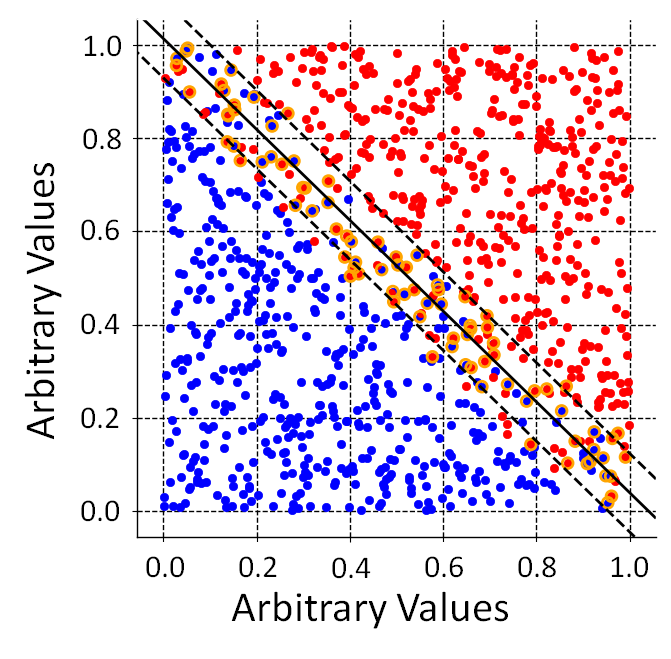
\includegraphics[width=\linewidth]{Chapter4/Figs/adjustedSvmPlots/adjusted_LinNoSepExample.png}
  \captionof{figure}[LIBSVM linear separation example (with overlap).]{How a support vector machine using LIBSVM trains on linear data with no separation. This is similar to how the neutron and noise data looks to the SVM in section \ref{sec:MachineLearningTrigger}.}
  \label{fig:LinNoSepExample}
\end{minipage}
\end{figure}

\begin{figure}[!h]
\centering
\begin{minipage}{.45\textwidth}
  \centering
  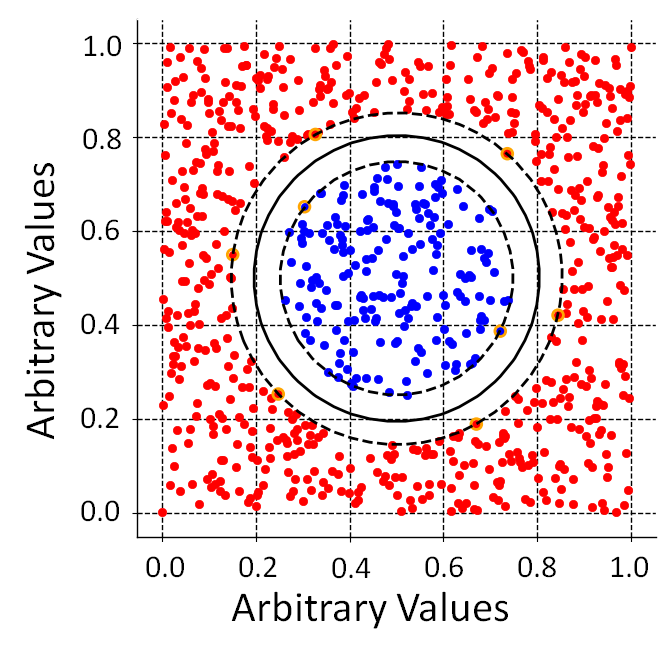
\includegraphics[width=\linewidth]{Chapter4/Figs/adjustedSvmPlots/adjusted_CircleSepExample.png}
  \captionof{figure}[LIBSVM circular separation example (no overlap)]{How the a support vector machine using LIBSVM trains on circular data with a separation.} 
  \label{fig:CircleSepExample}
\end{minipage}%
\qquad
\begin{minipage}{.45\textwidth}
  \centering
  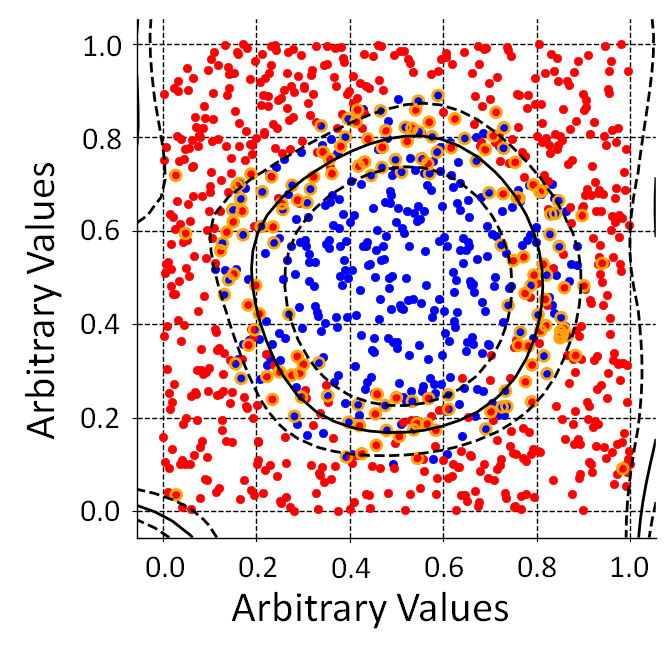
\includegraphics[width=\linewidth]{Chapter4/Figs/adjustedSvmPlots/adjusted_CircleNoSepExample.png}
  \captionof{figure}[LIBSVM circular separation example (with overlap)]{How the a support vector machine using LIBSVM trains on circular data with no separation.}
  \label{fig:CircleNoSepExample}
\end{minipage}
\end{figure}

\begin{figure}[!h]
 \centering
 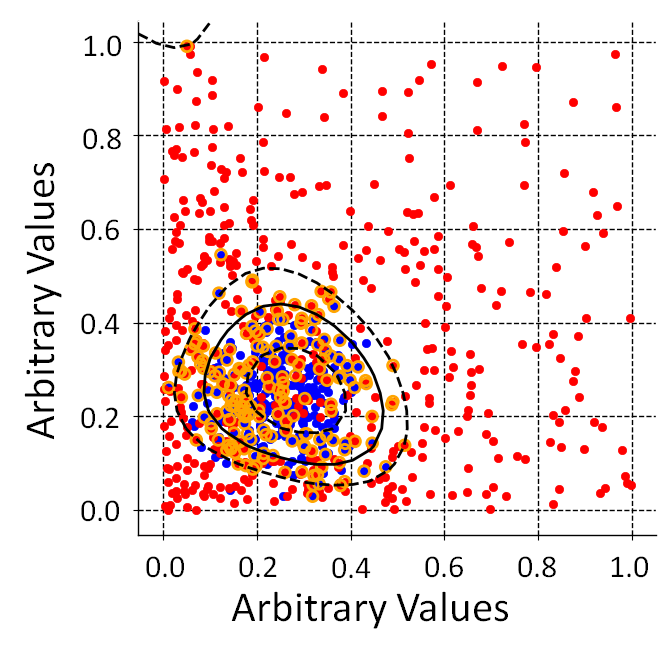
\includegraphics[width=0.5\linewidth]{Chapter4/Figs/adjustedSvmPlots/adjusted_exp_1GausseExample.png}
 \captionof{figure}[LIBSVM  exponential x,y noise and single Gaussian peak.]{How the a support vector machine using LIBSVM trains on data with only a single Gaussian peak and exponential noise in the x and y.} 
 \label{fig:exp_1GausseExample}
\end{figure}

\begin{figure}[!h]
 \centering
 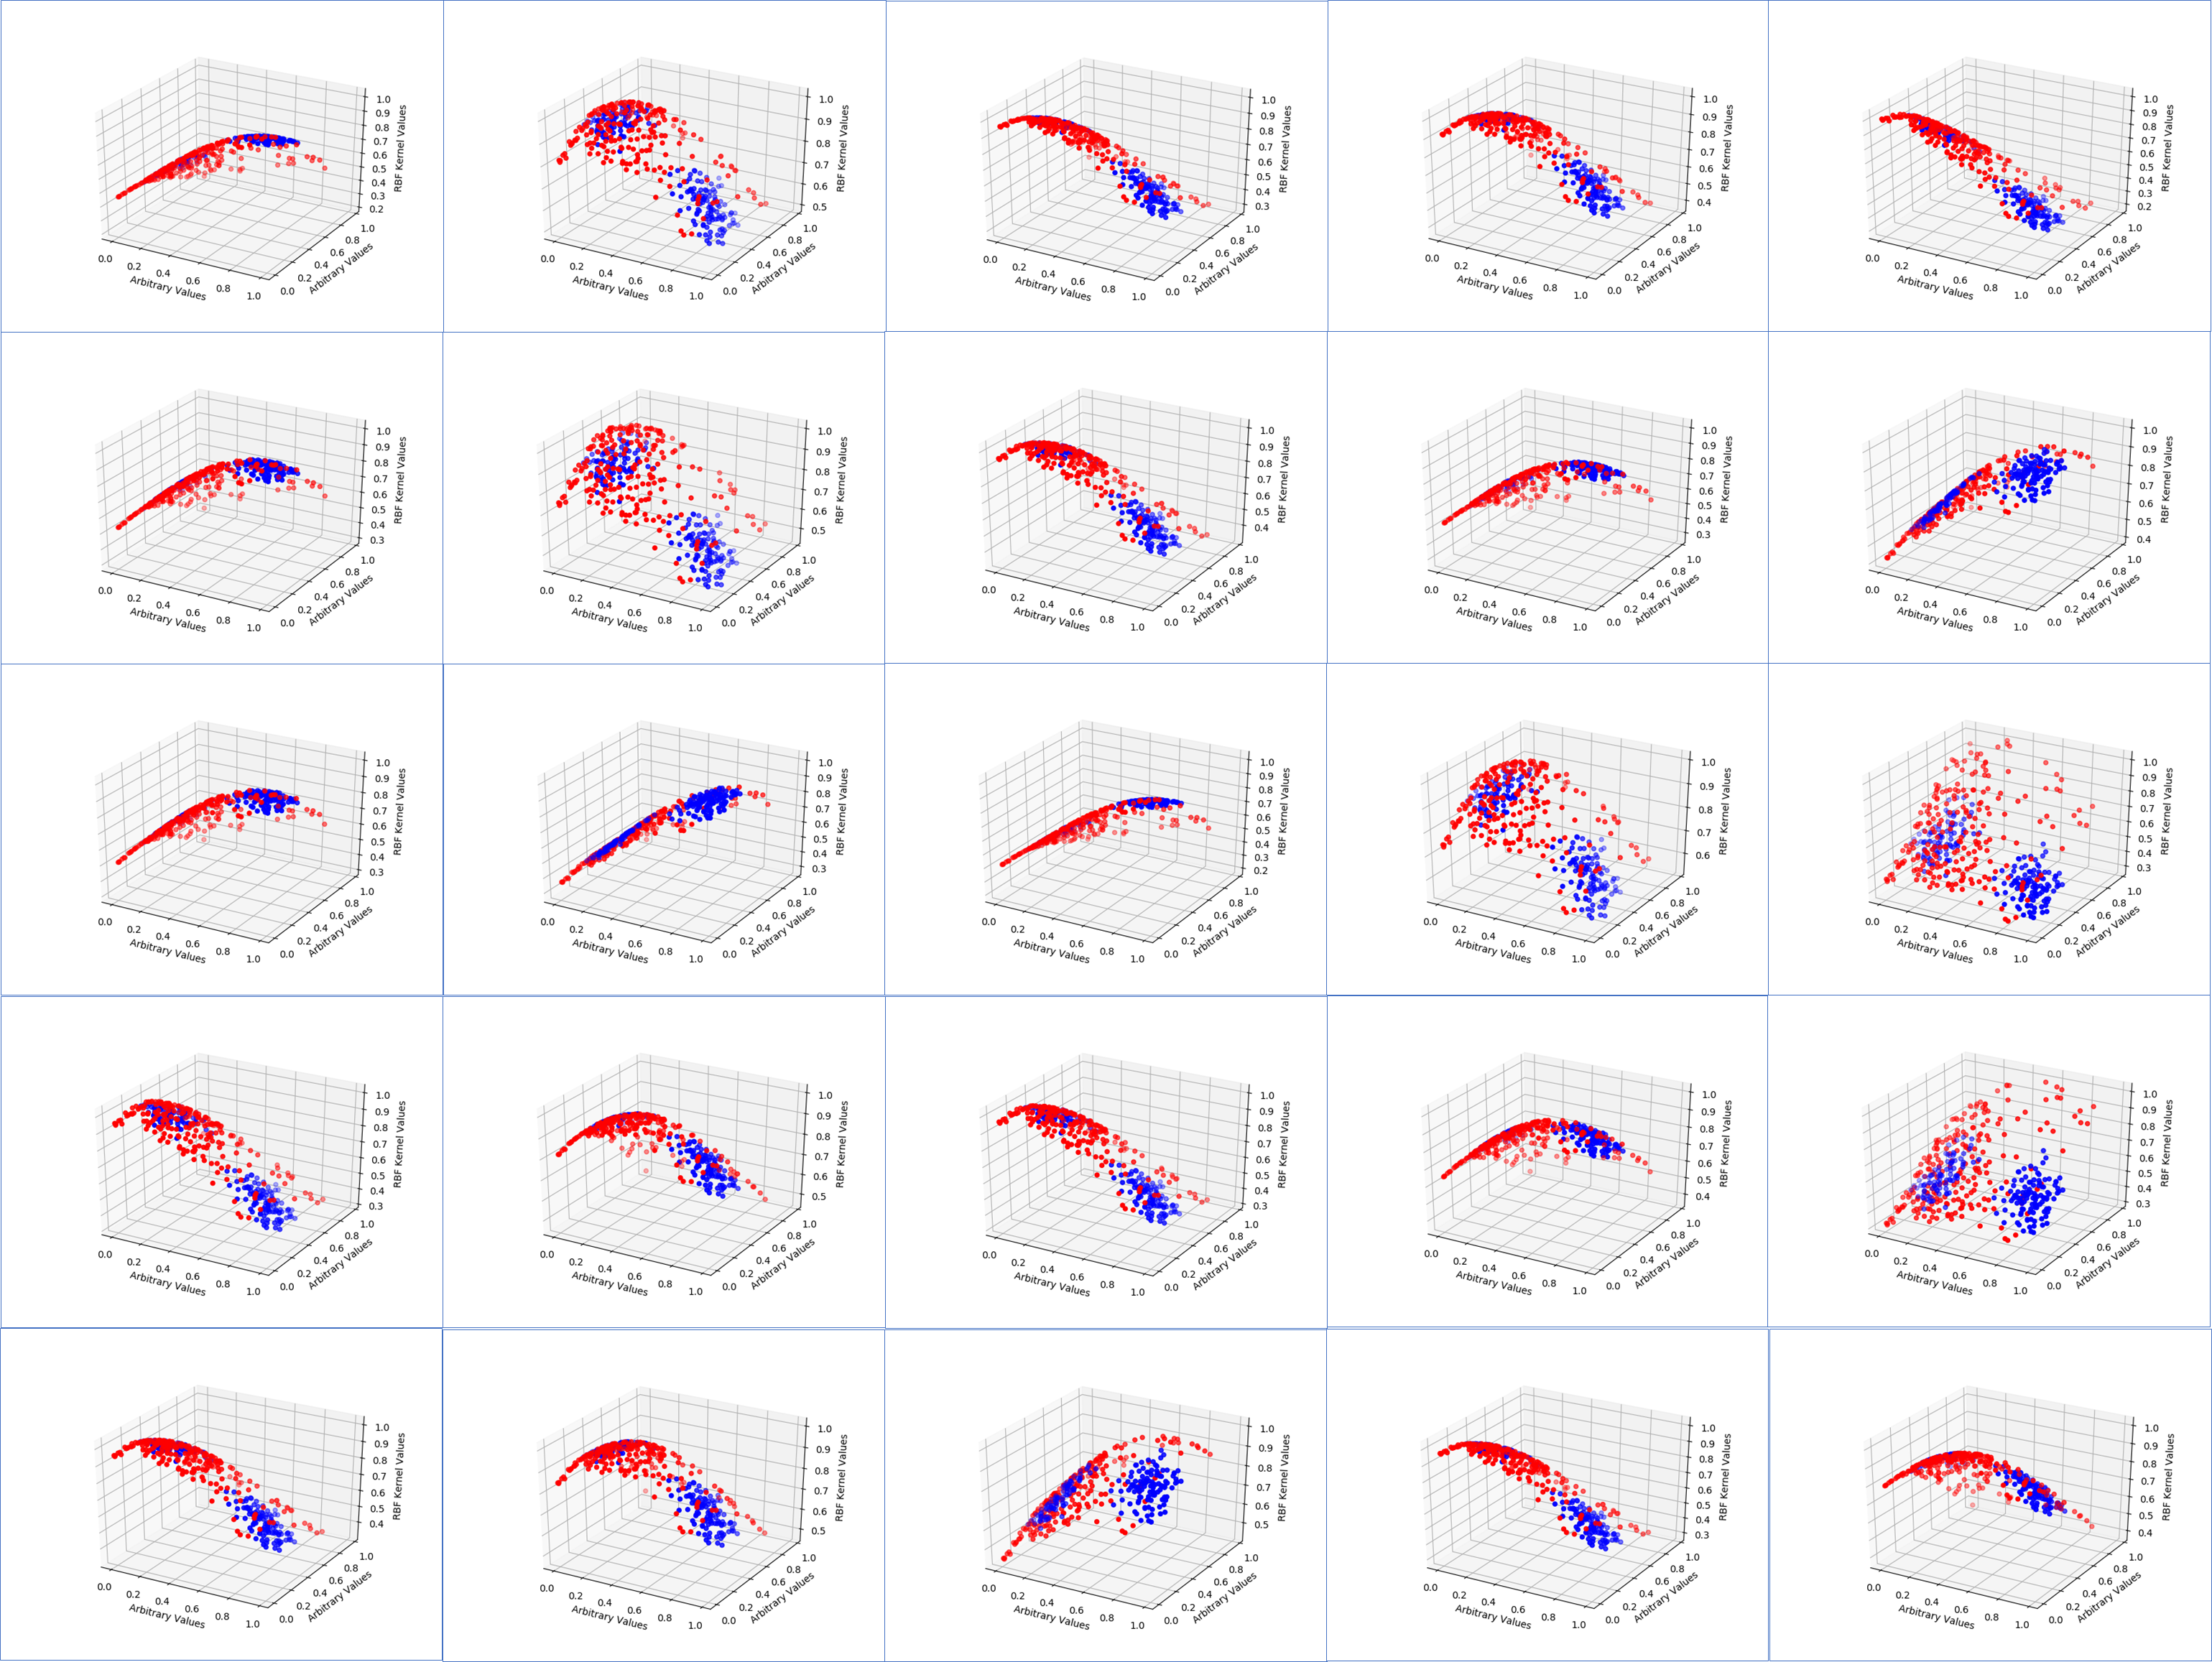
\includegraphics[width=\linewidth]{Appendix1/Figs/25OutOf425kSamples.png}
 \captionof{figure}[A Sample to show how the RBF kernel in figure \ref{fig:svmExp_GausseExamples} distorts the data to make it linearly separable.]{A Sample to show how the RBF kernel in figure \ref{fig:svmExp_GausseExamples} distorts the data to make it linearly separable. Every point in the training set (425 points) will be the maximum for a given slice and is distorted around. All of these slices are then analysed by the SVM at once. This figure represents the first 25 points that are distorted around. The SVM will view all of the 425 graphs simultaneously to form any complex boundary. But this causes the problem to jump from a n$^2$ computational problem (SVM alone) to an n$^3$ computational problem (SVM with kernel). } 
 \label{fig:25OutOf425kSamples}
\end{figure}

\begin{figure}[!h]
\centering
\begin{subfigure}{.5\textwidth}
  \centering
  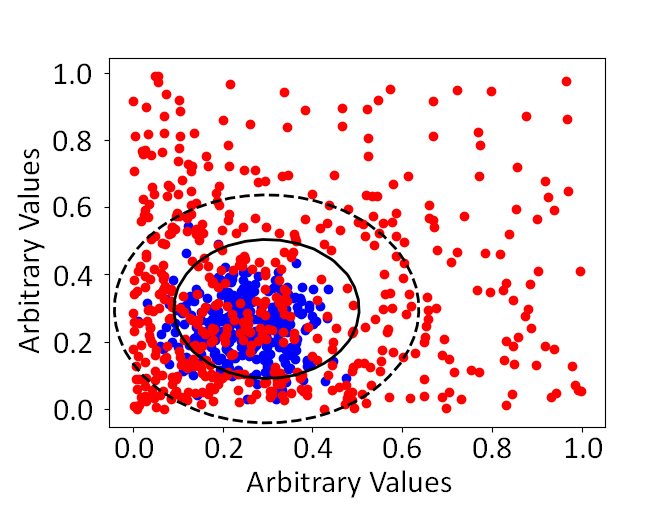
\includegraphics[width=\linewidth]{Appendix1/Figs/singleGaussExp_RbfPointDistortion.png}
  \captionsetup{width=.9\linewidth}
  \caption{}
  \label{subFig:singleGuassPointDist}
\end{subfigure}%
\begin{subfigure}{.5\textwidth}
  \centering
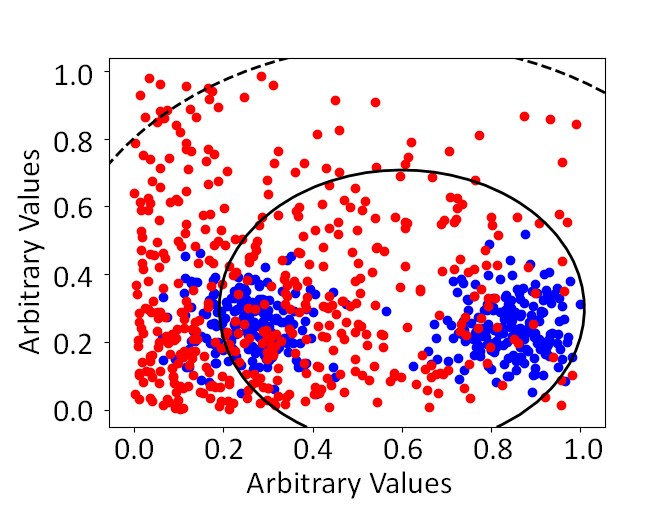
\includegraphics[width=\linewidth]{Appendix1/Figs/doubleGaussExp_RbfPointDistortion.png}
  \captionsetup{width=.9\linewidth}
  \caption{}
  \label{subFig:doubleGaussPointDist}
\end{subfigure}
\caption[RBF kernel distortion around a lone single point for an (x,y) Gaussian and double Gaussian case.]{How the RBF kernel distorts around a single point for a single Gaussian (a) and double Gaussian (b) case. When distorting around a single point only a circle can be made when projecting back into the 2D space. Both (a) and (b) show the best possible point to distort around and whilst the single Gaussian case is acceptable (a) the double Gaussian case is poor (b). }
\label{fig:GuassPointDist}
\end{figure}


\begin{figure}[!h]
\centering
\begin{subfigure}{.5\textwidth}
  \centering
  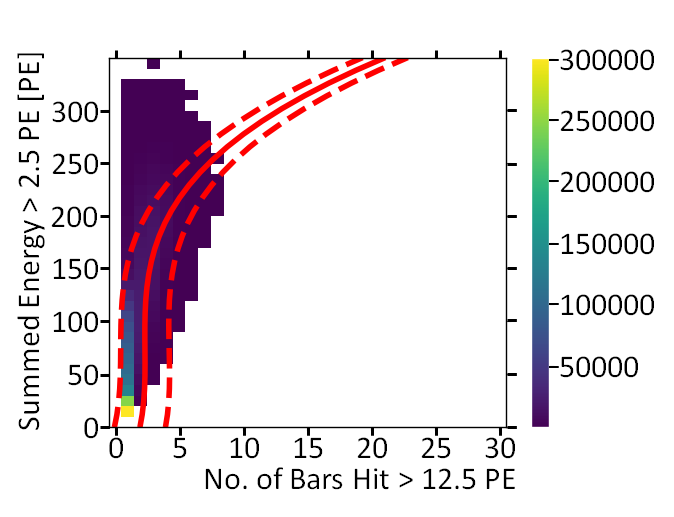
\includegraphics[width=\linewidth]{Appendix1/Figs/Bars2Sum1Noise.png}
  \captionsetup{width=.9\linewidth}
  \caption{}
  \label{subFig:Bars2Sum1Noise}
\end{subfigure}%
\begin{subfigure}{.5\textwidth}
  \centering
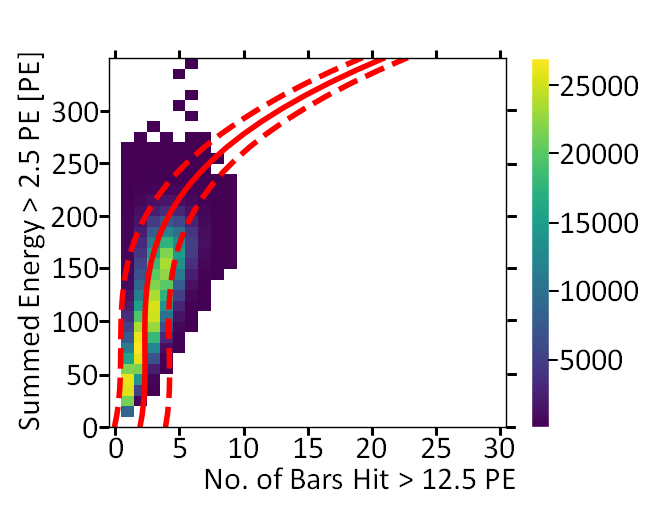
\includegraphics[width=\linewidth]{Appendix1/Figs/Bars2Sum1Signal.png}
  \captionsetup{width=.9\linewidth}
  \caption{}
  \label{subFig:Bars2Sum1Signal}
\end{subfigure}
\caption[LIBLINEAR SVM Nyström approximated RBF kernel for number of bars hit > 12.5\,PE vs summed energy > 2.5\,PE.]{How the SVM trains when using number of bars hit past 12.5\,PE and summed energy when each hit has a threshold of 2.5\,PE. C = 10$^6$ $\gamma$ = 10$^{-6}$. (a) Shows noise (b) shows the neutron signal. The boundary has strong linearity for most events but curves at the edges. Efficiency = 50.0\,\%,, purity 79.9\,\%.}
\label{fig:Bars2Sum1SignalNoise}
\end{figure}

\begin{figure}[!h]
\centering
\begin{subfigure}{.5\textwidth}
  \centering
  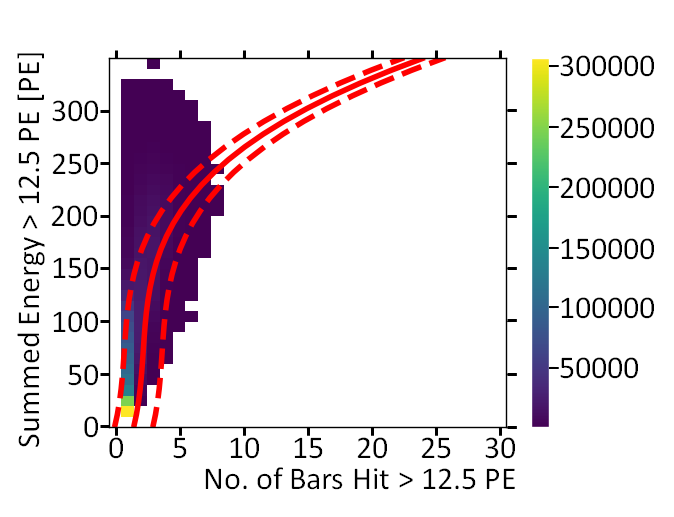
\includegraphics[width=\linewidth]{Appendix1/Figs/Bars2Sum2Noise.png}
  \captionsetup{width=.9\linewidth}
  \caption{}
  \label{subFig:Bars2Sum2N}
\end{subfigure}%
\begin{subfigure}{.5\textwidth}
  \centering
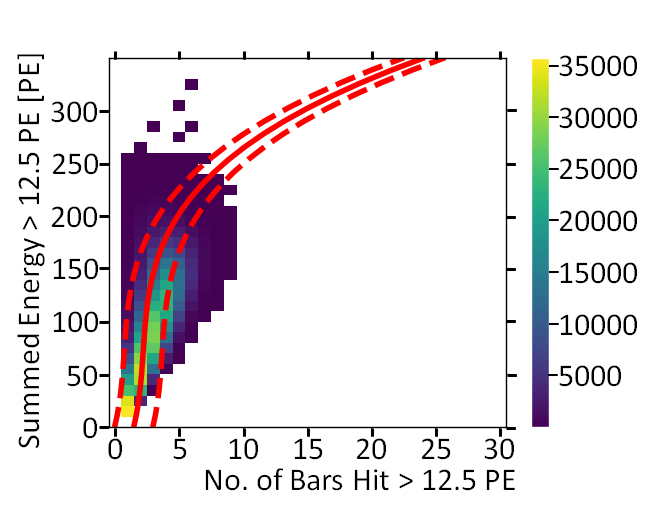
\includegraphics[width=\linewidth]{Appendix1/Figs/Bars2Sum2Signal.png}
  \captionsetup{width=.9\linewidth}
  \caption{}
  \label{subFig:Bars2Sum2S}
\end{subfigure}
\caption[LIBLINEAR SVM Nyström approximated RBF kernel for number of bars hit > 12.5\,PE vs summed energy > 12.5\,PE.]{How the SVM trains when using number of bars hit past 12.5\,PE and summed energy when each hit has a threshold of 12.5\,PE. C = 10$^6$ $\gamma$ = 10$^{-6}$. (a) Shows noise (b) shows the neutron signal. The boundary has strong linearity for most events but curves at the edges. Efficiency = 54.8\,\%,, purity 85.1\,\%.}
\label{fig:Bars2Sum2SN}
\end{figure}

\begin{figure}[!h]
\centering
\begin{subfigure}{.5\textwidth}
  \centering
  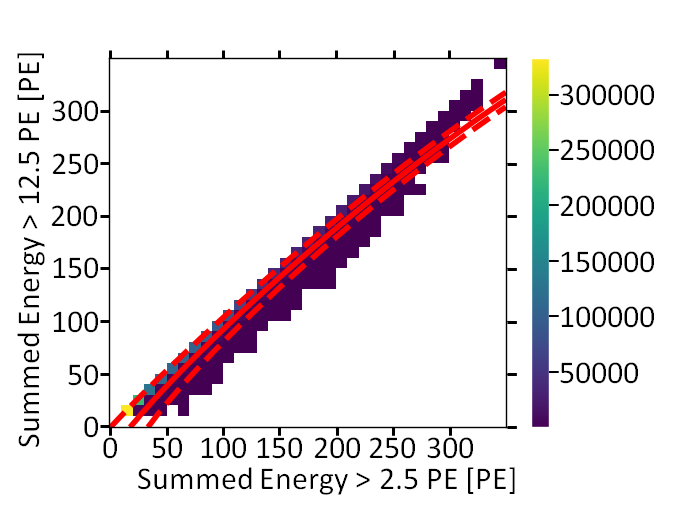
\includegraphics[width=\linewidth]{Appendix1/Figs/Sum1Sum2Noise.png}
  \captionsetup{width=.9\linewidth}
  \caption{}
  \label{subFig:Sum1Sum2N}
\end{subfigure}%
\begin{subfigure}{.5\textwidth}
  \centering
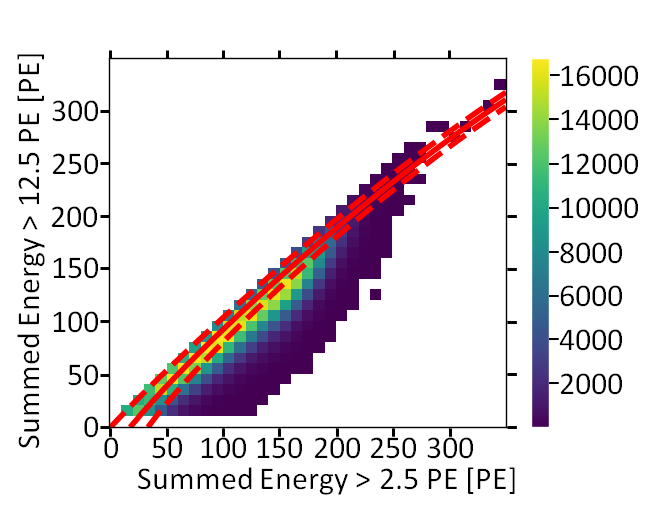
\includegraphics[width=\linewidth]{Appendix1/Figs/Sum1Sum2Signal.png}
  \captionsetup{width=.9\linewidth}
  \caption{}
  \label{subFig:Sum1Sum2S}
\end{subfigure}
\caption[LIBLINEAR SVM Nyström approximated RBF kernel for summed energy > 12.5\,PE vs summed energy > 2.5\,PE.]{How the SVM trains when using summed energy when each hit has a threshold 2.5\,PE and summed energy with a hit threshold of 12.5\,PE. C = 10$^6$ $\gamma$ = 10$^{-6}$. (a) Shows noise (b) shows the neutron signal. The boundary has strong linearity and curves very slightly at the edge. Efficiency = 67.9\,\%,, purity 90.4\,\%.}
\label{fig:Sum1Sum2SN}
\end{figure}

\begin{figure}[!h]
\centering
\begin{subfigure}{.5\textwidth}
  \centering
  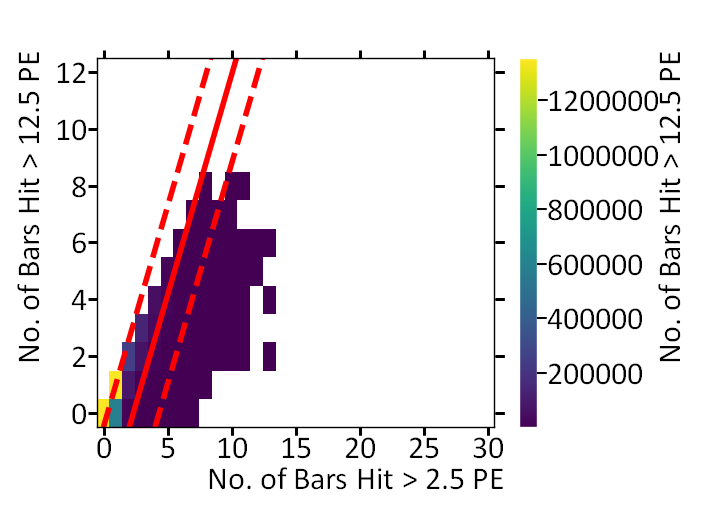
\includegraphics[width=\linewidth]{Appendix1/Figs/Bars1Bars2Noise.png}
  \captionsetup{width=.9\linewidth}
  \caption{}
  \label{subFig:Bars1Bars2N}
\end{subfigure}%
\begin{subfigure}{.5\textwidth}
  \centering
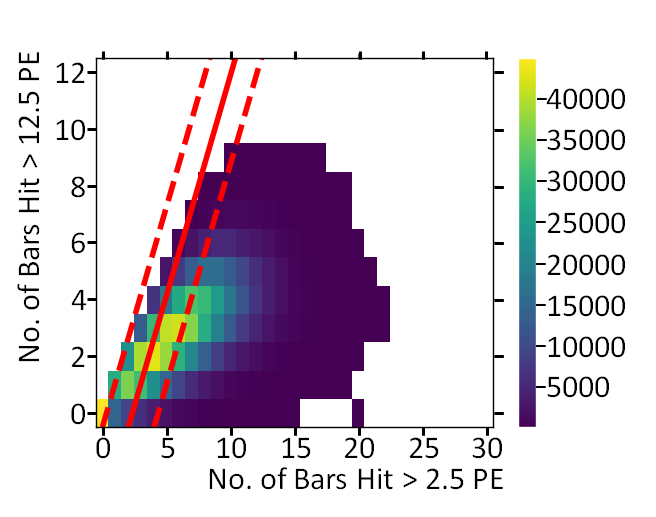
\includegraphics[width=\linewidth]{Appendix1/Figs/Bars1Bars2Signal.png}
  \captionsetup{width=.9\linewidth}
  \caption{}
  \label{subFig:Bars1Bar2S}
\end{subfigure}
\caption[LIBLINEAR SVM Nyström approximated RBF kernel for number of bars hit > 12.5\,PE vs number of bars hit > 2.5\,PE.]{How the SVM trains when using number of bars hit past 2.5\,PE and number of bars past 12.5\,PE. C = 10$^6$ $\gamma$ = 10$^{-6}$. (a) Shows noise (b) shows the neutron signal. The boundary is entirely linear. Efficiency = 75.3\,\%,, purity 91.7\,\%.}
\label{fig:Bars1BarsSN}
\end{figure}

\begin{figure}[!h]
\centering
\begin{subfigure}{.5\textwidth}
  \centering
  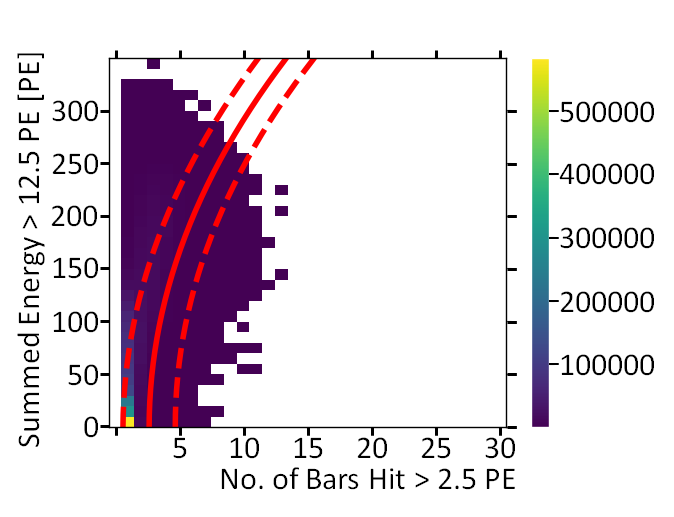
\includegraphics[width=\linewidth]{Appendix1/Figs/Bars1Sum2Noise.png}
  \captionsetup{width=.9\linewidth}
  \caption{}
  \label{subFig:Bars1Sum2N}
\end{subfigure}%
\begin{subfigure}{.5\textwidth}
  \centering
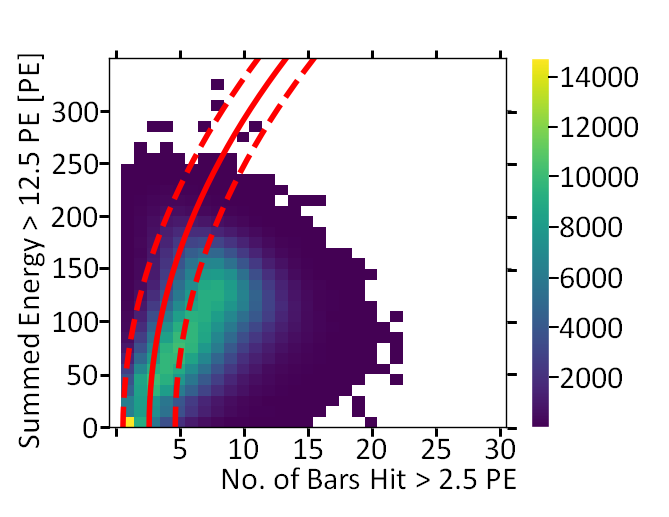
\includegraphics[width=\linewidth]{Appendix1/Figs/Bars1Sum2Signal.png}
  \captionsetup{width=.9\linewidth}
  \caption{}
  \label{subFig:Bars1Sum2S}
\end{subfigure}
\caption[LIBLINEAR SVM Nyström approximated RBF kernel for number of bars hit > 2.5\,PE vs summed energy > 12.5\,PE.]{How the SVM trains when using number of bars hit past 2.5\,PE and summed energy when each hit has a threshold of 12.5\,PE. C = 10$^6$ $\gamma$ = 10$^{-6}$. (a) Shows noise (b) shows the neutron signal. The boundary has reasonable linearity for most events but curves at the edge. Efficiency = 78.5\,\%,, purity 94.8\,\%.}
\label{fig:Bars1Sum2SN}
\end{figure}

\begin{figure}[!h]
\centering
\begin{subfigure}{.5\textwidth}
  \centering
  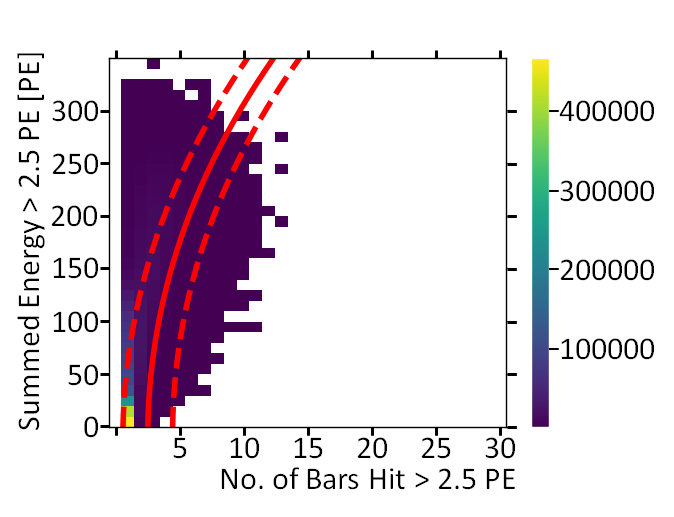
\includegraphics[width=\linewidth]{Appendix1/Figs/Bars1Sum1Noise.png}
  \captionsetup{width=.9\linewidth}
  \caption{}
  \label{subFig:Bars1Sum1N}
\end{subfigure}%
\begin{subfigure}{.5\textwidth}
  \centering
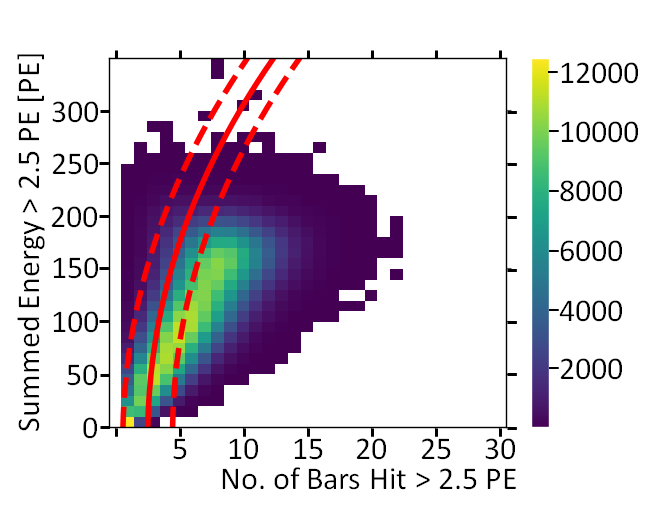
\includegraphics[width=\linewidth]{Appendix1/Figs/Bars1Sum1Signal.png}
  \captionsetup{width=.9\linewidth}
  \caption{}
  \label{subFig:Bars1Sum1S}
\end{subfigure}
\caption[LIBLINEAR SVM Nyström approximated RBF kernel for number of bars hit > 2.5\,PE vs summed energy > 2.5\,PE.]{How the SVM trains when using number of bars hit past 2.5\,PE and summed energy when each hit has a threshold of 2.5\,PE. C = 10$^6$ $\gamma$ = 10$^{-6}$. (a) Shows noise (b) shows the neutron signal. The boundary has reasonable linearity for most events but curves at the edge. Efficiency = 78.5\,\%,, purity 94.8\,\%.}
\label{fig:Bars1Sum1SN}
\end{figure}

\begin{figure}[!h]
\centering
\begin{minipage}{.45\textwidth}
  \centering
  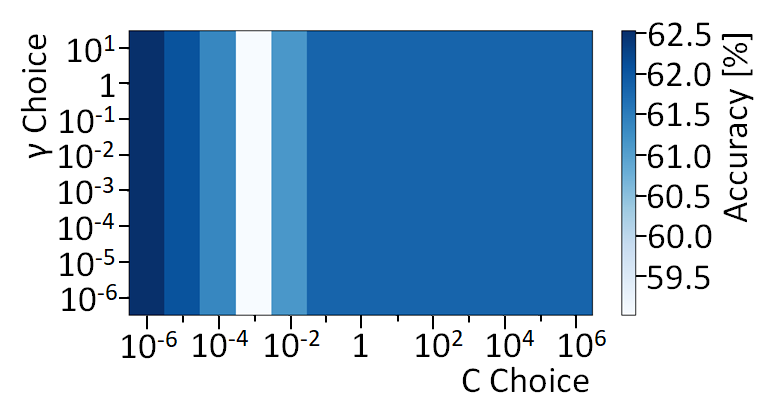
\includegraphics[width=\linewidth]{Appendix1/Figs/exp2GaussLinearGridSearch.png}
  \captionof{figure}[LIBLINEAR SVM C and $\gamma$ grid search for the x,y double Gaussian data set.]{An SVM grid search for a linear SVM when training on the 2 Gaussian signal distributions and exp noise in the x and y this is not very linearly separable and the SVM struggles without a kernel it is 22.5\,\% less accurate than with the RBF kernel.} 
  \label{fig:exp2GaussLinearGridSearch}
  %\vspace{0.478cm} %0.478cm per line
\end{minipage}%
\qquad
\begin{minipage}{.45\textwidth}
  \centering
  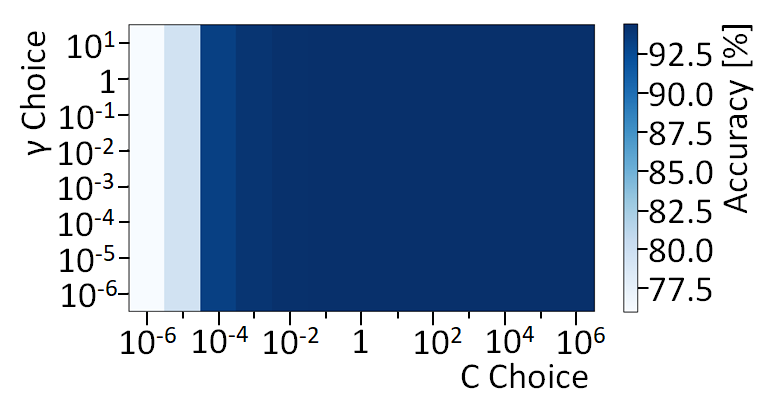
\includegraphics[width=\linewidth]{Appendix1/Figs/NeutronNoiseLinearGridSearch.png}
  \captionof{figure}[LIBLINEAR SVM C and $\gamma$ grid search for the neutron data set when using all 4 variables.]{An SVM grid search for a linear SVM when using the generated neutron data and noise data with 2.5\,PE and 12.5\,PE thresholds. It is very linearly separable and it is only 0.5\,\% less accurate than with the RBF kernel (94.38\,\% vs 94.87\,\%).}
  \label{fig:NeutronNoiseLinearGridSearch}
\end{minipage}
\end{figure}

\begin{figure}[!h]
\centering
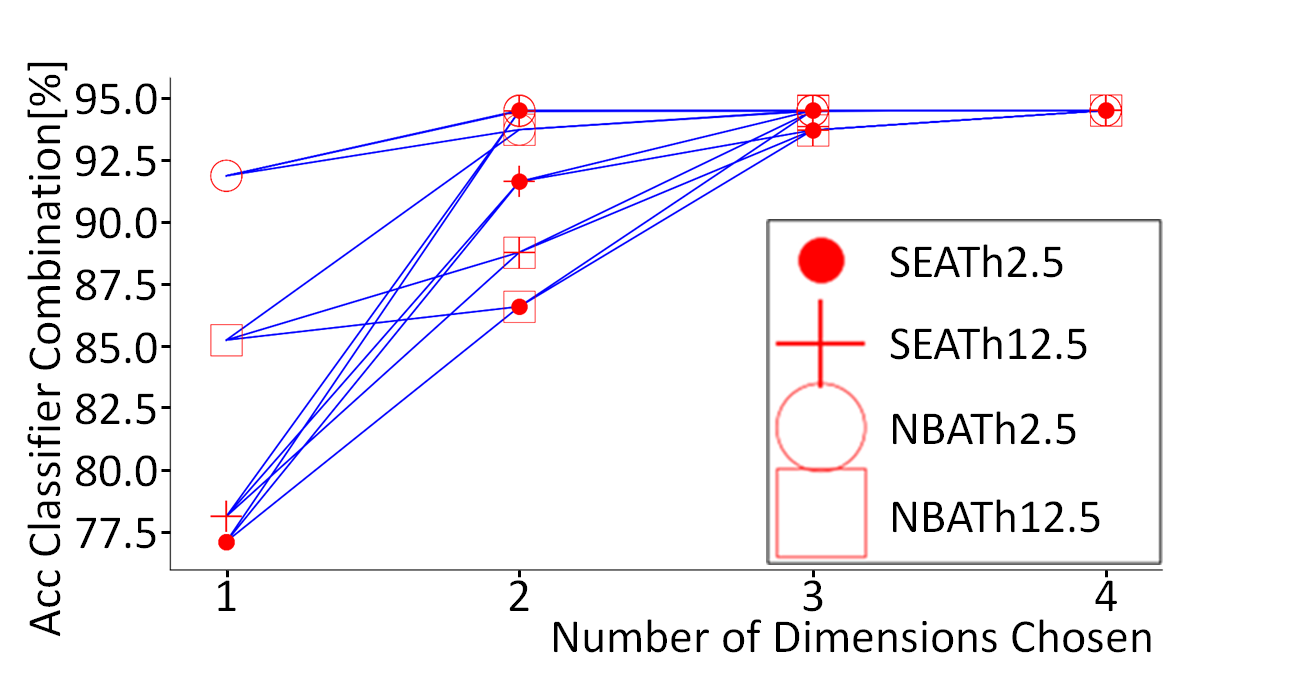
\includegraphics[width=0.8\linewidth]{Appendix1/Figs/accLinNeutronSVMC1e6_g1e-6MedText.png}
\captionof{figure}[LIBLINEAR SVM accuracy (no kernel) for generated neutron data.]{Linear SVM accuracy (no kernel) separating 1 million generated neutron signal events and generated 4 million noise events. It is mostly the same as the RBF kernel SVM but the optimum combination is 0.5\,\% lower.} 
\label{fig:accLinNeutronSVMC1e6_g1e-6MedText}
\end{figure}

\begin{figure}[!h]
\centering
\begin{minipage}{.45\textwidth}
  \centering
  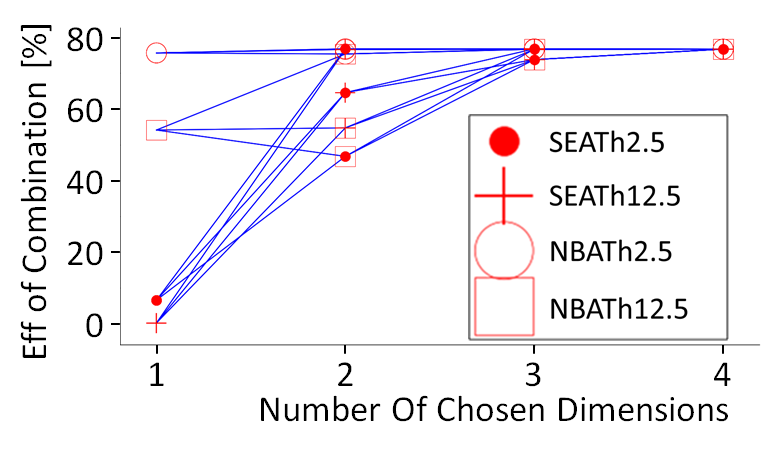
\includegraphics[width=\linewidth]{Appendix1/Figs/effLinCombSVMAdjustMedText.png}
  \captionof{figure}[LIBLINEAR SVM efficiency (no kernel) for generated neutron data.]{Linear SVM efficiency (no kernel) separating 1 million generated neutron signal events and generated 4 million noise events. It is mostly the same as the RBF kernel SVM but the optimum combination does not improve past 1D.} 
  \label{fig:effLinCombSVMAdjustMedText}
\end{minipage}%
\qquad
\begin{minipage}{.45\textwidth}
  \centering
  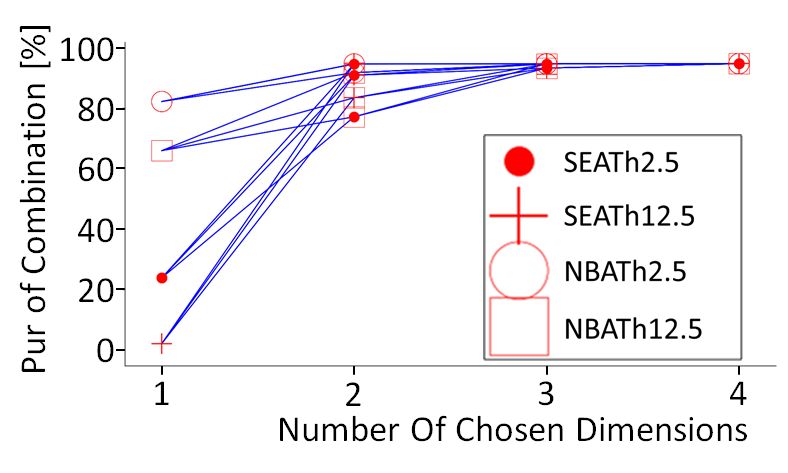
\includegraphics[width=\linewidth]{Appendix1/Figs/purLinCombSVMAdjustMedText.png}
  \captionof{figure}[LIBLINEAR SVM (no kernel) purity for generated neutron data.]{Linear SVM purity (no kernel) separating 1 million generated neutron signal events and generated 4 million noise events. It is mostly the same as the RBF kernel SVM.}
  \label{fig:purLinCombSVMAdjustMedText}
  \vspace{0.956cm} %0.478cm per line
\end{minipage}
\end{figure}

% \section*{Windows OS}

% \subsection*{TeXLive package - full version}
% \begin{enumerate}
% \item	Download the TeXLive ISO (2.2GB) from\\
% \href{https://www.tug.org/texlive/}{https://www.tug.org/texlive/}
% \item	Download WinCDEmu (if you don't have a virtual drive) from \\
% \href{http://wincdemu.sysprogs.org/download/}
% {http://wincdemu.sysprogs.org/download/}
% \item	To install Windows CD Emulator follow the instructions at\\
% \href{http://wincdemu.sysprogs.org/tutorials/install/}
% {http://wincdemu.sysprogs.org/tutorials/install/}
% \item	Right click the iso and mount it using the WinCDEmu as shown in \\
% \href{http://wincdemu.sysprogs.org/tutorials/mount/}{
% http://wincdemu.sysprogs.org/tutorials/mount/}
% \item	Open your virtual drive and run setup.pl
% \end{enumerate}

% \begin{table}
% \caption{A nice looking table}
% \centering
% \label{table:nice_table}
% \begin{tabular}{l c c c c}
% \hline 
% \multirow{2}{*}{Dental measurement} & \multicolumn{2}{c}{Species I} & \multicolumn{2}{c}{Species II} \\ 
% \cline{2-5}
%   & mean & SD  & mean & SD  \\ 
% \hline
% I1MD & 6.23 & 0.91 & 5.2  & 0.7  \\

% I1LL & 7.48 & 0.56 & 8.7  & 0.71 \\

% I2MD & 3.99 & 0.63 & 4.22 & 0.54 \\

% I2LL & 6.81 & 0.02 & 6.66 & 0.01 \\

% CMD & 13.47 & 0.09 & 10.55 & 0.05 \\

% CBL & 11.88 & 0.05 & 13.11 & 0.04\\ 
% \hline 
% \end{tabular}
% \end{table}


% \begin{table}
% \caption{Even better looking table using booktabs}
% \centering
% \label{table:good_table}
% \begin{tabular}{l c c c c}
% \toprule
% \multirow{2}{*}{Dental measurement} & \multicolumn{2}{c}{Species I} & \multicolumn{2}{c}{Species II} \\ 
% \cmidrule{2-5}
%   & mean & SD  & mean & SD  \\ 
% \midrule
% I1MD & 6.23 & 0.91 & 5.2  & 0.7  \\

% I1LL & 7.48 & 0.56 & 8.7  & 0.71 \\

% I2MD & 3.99 & 0.63 & 4.22 & 0.54 \\

% I2LL & 6.81 & 0.02 & 6.66 & 0.01 \\

% CMD & 13.47 & 0.09 & 10.55 & 0.05 \\

% CBL & 11.88 & 0.05 & 13.11 & 0.04\\ 
% \bottomrule
% \end{tabular}
% \end{table}


